\begin{block}{System Architecture}
\begin{multicols}{2}
\centering
\alert{Baseline} \\[0.5\baselineskip]
\includegraphics[scale=1.45]{img/system-base.pdf}

\columnbreak

\centering
\alert{Enhanced} \\[0.5\baselineskip]
\includegraphics[scale=1.45]{img/system-kvstore.pdf}
\end{multicols}
\end{block}

\vspace{1ex}

\begin{block}{Accelerator}
\footnotesize

\begin{multicols}{2}
\begin{center}
    \alert{Accelerator} \\[0.5\baselineskip]
    \includegraphics[width=\linewidth]{img/kvstore.pdf}
\end{center}

\columnbreak

\begin{center}
    \alert{Traffic Manager} \\[0.5\baselineskip]
    \includegraphics[width=\linewidth]{img/frontend.pdf}
\end{center}

\end{multicols}

\begin{itemize}
    \item The accelerator accepts a key and computes primary and secondary
        hash values, which it uses to retrieve the value from its local
        block RAM.
    \item The traffic manager, interposed between the NIC and the DMA
        engine, implements the specialized Memcached logic.
	For intercepted Memcached GET requests, it queries the
	accelerator and constructs the response packet if the key is found.
	Unhandled frames are forwarded to the DMA engine for processing
	by the operating system.
\end{itemize}
\end{block}

\vspace{1ex}

\begin{block}{DMA Engine}
\begin{itemize}
\footnotesize
\item Performs uncached memory accesses via the TileLink protocol
\item Transfers a \SI{512}{\bit} cache block per request
\item Front-end/back-end decoupling allows load prefetching to hide
	memory latency
\item Buffer descriptor rings exposed as queues through processor
	control registers
\end{itemize}

\begin{multicols}{2}
\centering
\includegraphics[scale=2.2]{img/dma-tx.pdf}

\columnbreak

\centering
\includegraphics[scale=2.2]{img/dma-rx.pdf}
\end{multicols}
\end{block}
